\section{Preliminaries}

We begin by exploring the strategies and tools for finding an optimal SRRL. The Pick-Up-Sticks algorithm will detail the basic structure used to find an SRRL, but not necessarily the optimal SRRL. Then we will explain the concept of equivalence classes, which can be grouped into segments. All of these concepts will be put together in our algorithm for finding the optimal solution.


\subsection{The Maximum Pick-Up-Sticks (MPUS) Algorithm}

As proposed by "Applegate et al."'s paper, we can build an algorithm for finding whether a pattern is a strip-rule pattern and, if so, finding an SRRL that generates it.

\subsubsection{The Pick-Up-Sticks (PUS) Algorithm.}

The Pick-Up-Sticks algorithm of \cite{ACJKLW07}
 is an algorithm for generating a SRRL of a pattern P if such a list exists. The idea is to pick up monochromatic rows and columns in order to build the SRRL backwards. Every time we pick a row or column, we color it gray.

Let $P$ be a black and white pattern. We define a column or row in P as being pseudo-monochromatic if it is composed of only gray and white cells or black and gray cells. Note that monochromatic columns and rows are also pseudo-monochromatic.

The Pick-Up-Sticks algorithm builds an SRRL as follows:

While there are still
black cells, choose a pseudo-monochromatic column or row and color all its cells gray. After a row or column is colored gray, add a rectangle that corresponds to covering that row or column with whatever non-gray color was left in that row or column to the beginning of our SRRL.
Note that, in our problem definition,
 we begin applying SRRLs with a white grid, so we can stop
picking up sticks when no black cells exist.
If, on the other hand, we modify the problem to begin with a grid of some
third color, we would only stop picking up sticks when all cells are gray.
There may be a difference of one rule between the optimum solutions to these two
problems (white grid or some third color grid) with the same target pattern.
For the sake of symmetry, from now on we use this {\em modified version}
of the problem. The method works with minor modifications for
the original version.

The algorithm may not succeed,
as it may not find a pseudo-monochromatic column or row.
If the algorithm does end in a all-gray grid,
%the algorithm has found a SRRL for the pattern $P$. If not, $P$ is not a strip-rule pattern. For the successful case,
the algorithm has "picked up" the rectangles of the SRRL in reverse order. Figure~\ref{fig:pick_up_sticks_example} gives a representation of one possible execution of the Pick-Up-Sticks algorithm and Fig.~\ref{fig:pick_up_sticks_srrl} shows the generation of the original pattern from the resultant SRRL.

\begin{figure}[h]
\centering
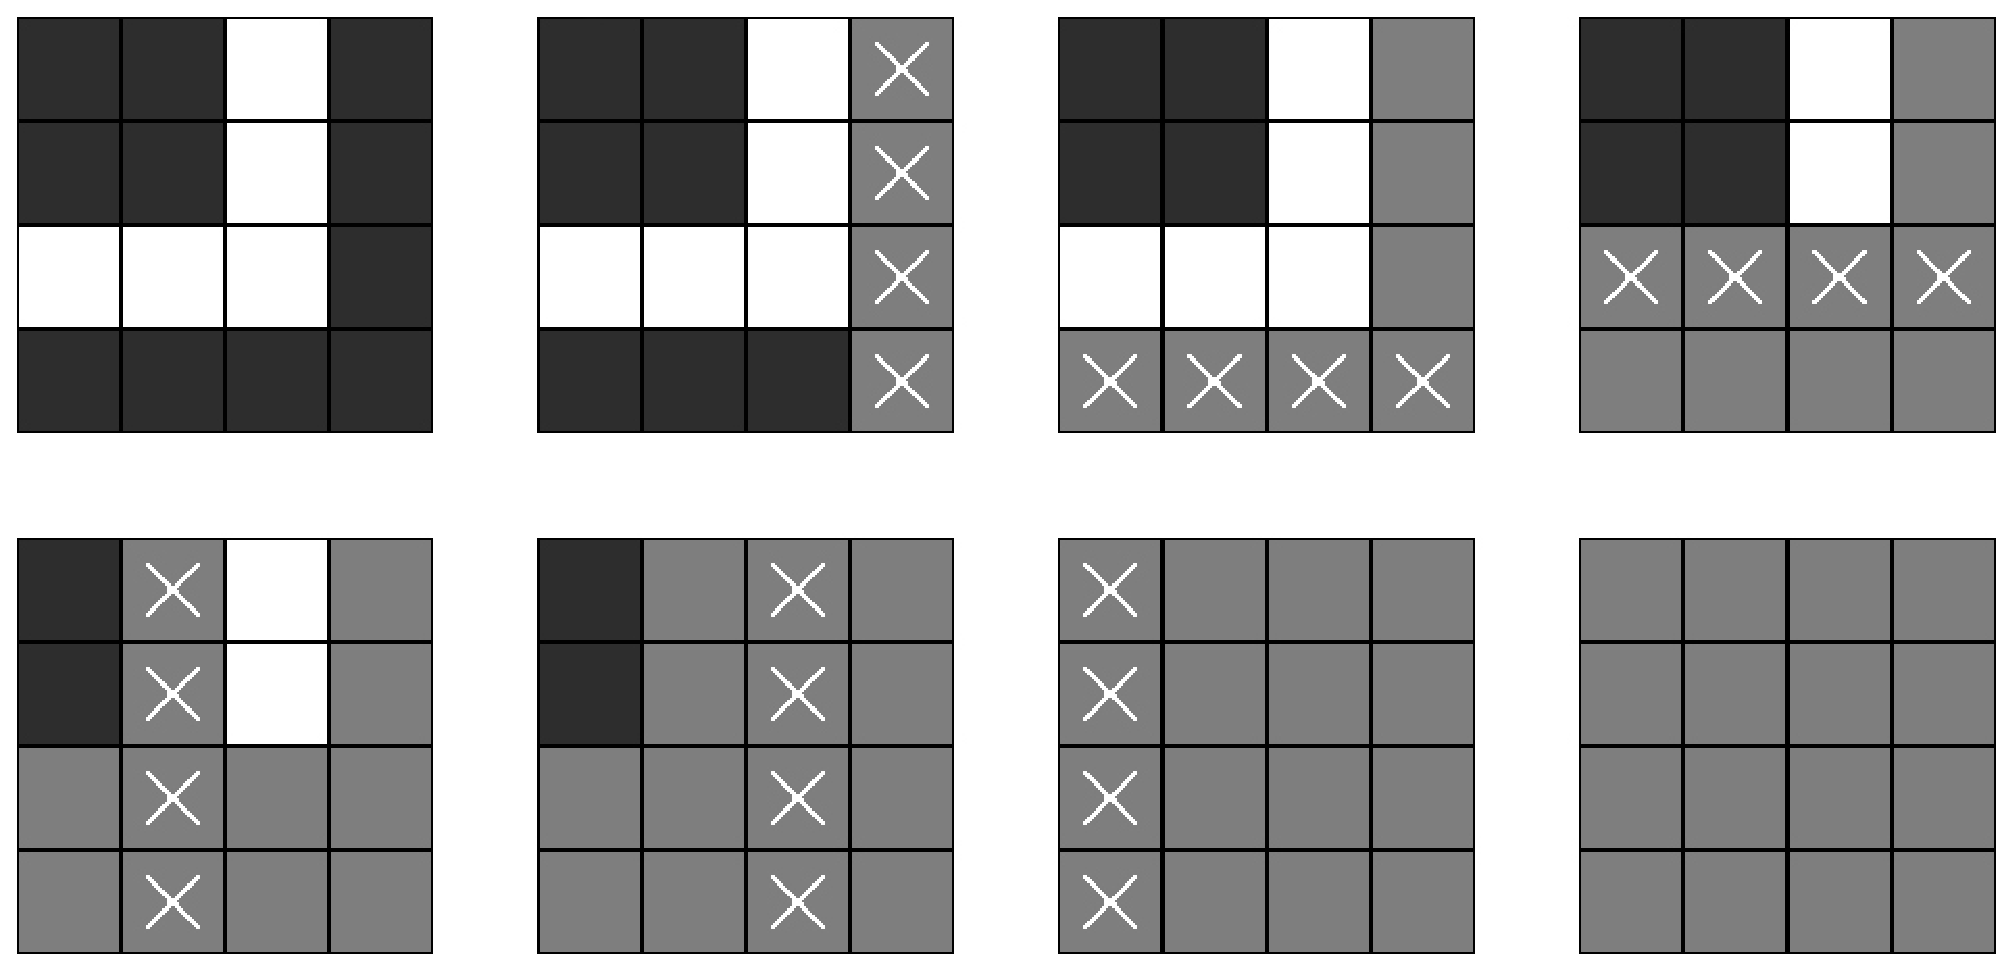
\includegraphics[width=10cm]{pick_up_sticks_example}
\caption{The execution of the Pick-Up-Sticks algorithm on a strip-rule pattern.}
\label{fig:pick_up_sticks_example}
\end{figure}

\begin{figure}[h]
\centering
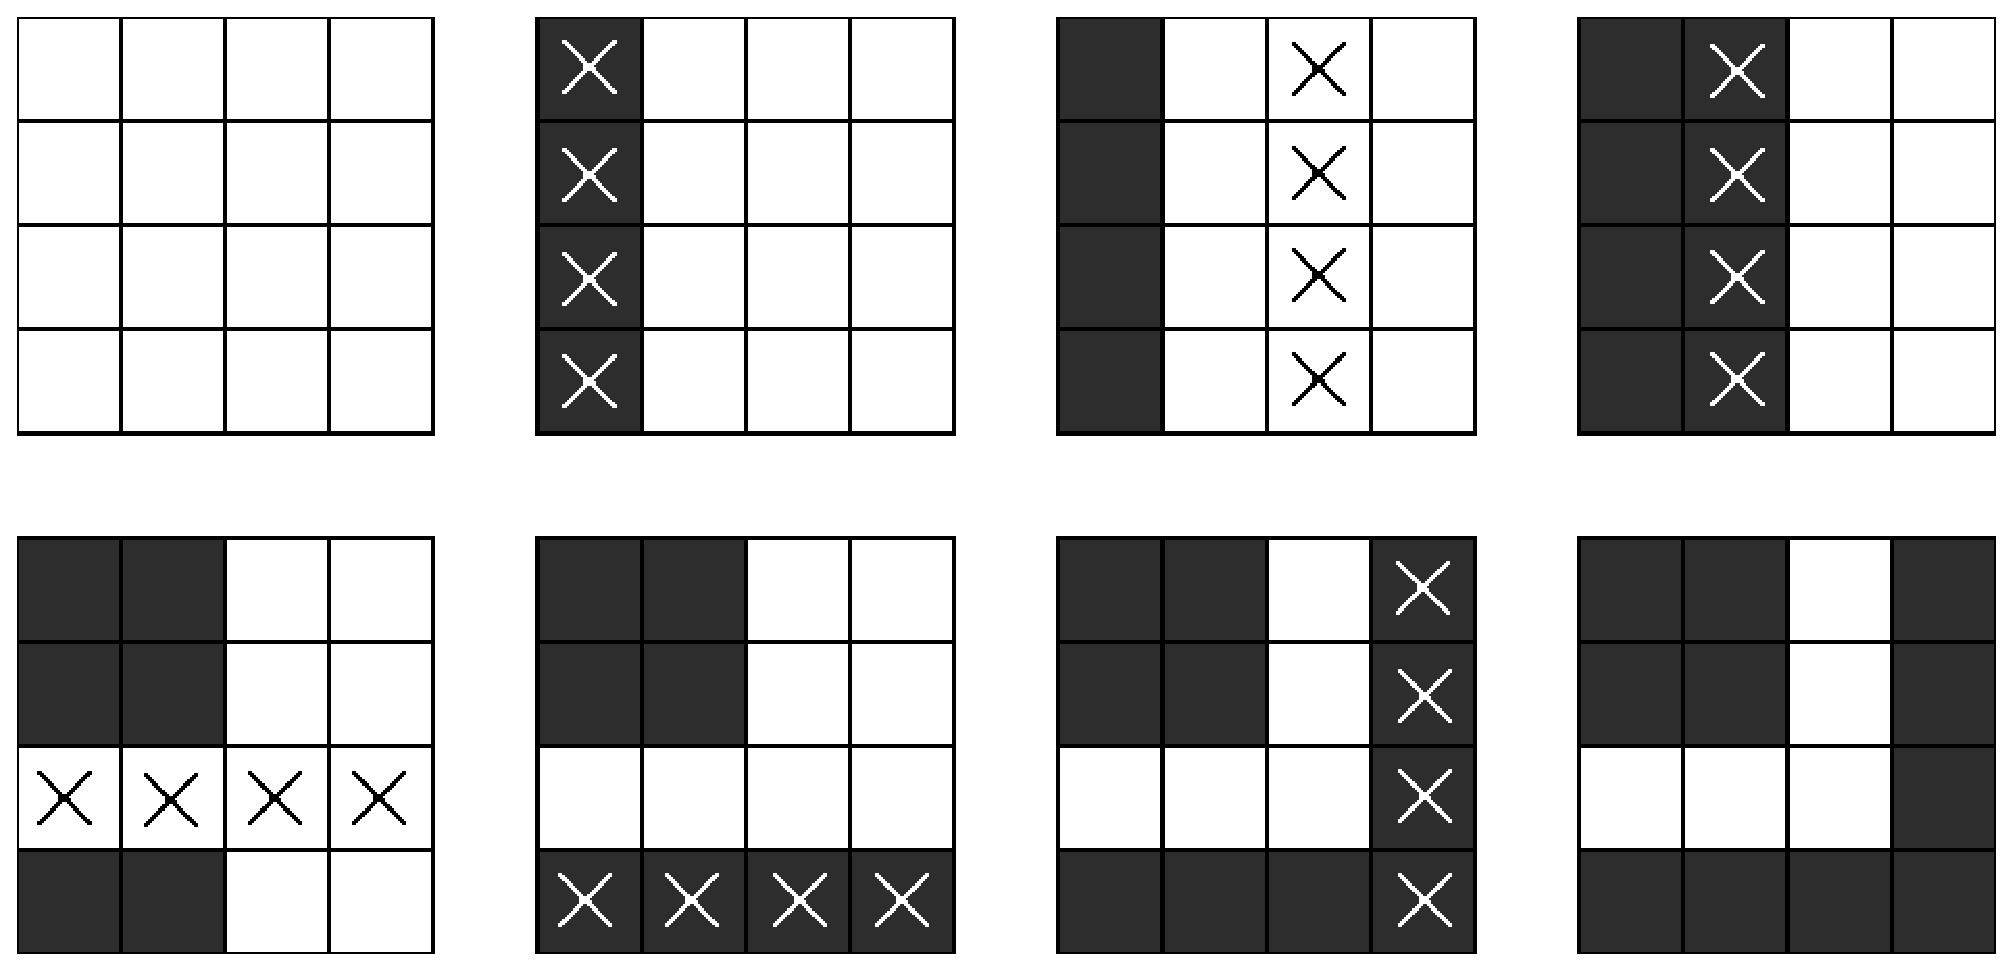
\includegraphics[width=10cm]{pick_up_sticks_srrl}
\caption{The SRRL generated by the execution of the MPUS algorithm on the pattern of the Figure~\ref{fig:pick_up_sticks_example}.}
\label{fig:pick_up_sticks_srrl}
\end{figure}

The Pick-Up-Sticks algorithm is guaranteed to generate an SRRL if one exists
\cite{ACJKLW07} (included in Appendix, Subsection \ref{corr_pus}), but it is not necessarily the optimal SRRL of minimum length. At any stage of the algorithm there will be more than one option on which row or column to pick up. Different choices can lead to different sizes of SRRLs. In the next sections we will discuss on how "Applegate et al."'s paper narrows down the number of choices for each stage in order to find the minimal SRRL.

\subsubsection{Improving by Picking Maximal Sticks.}

One important observation by "Applegate et al."'s paper on the Pick-Up-Sticks (PUS) algorithm is that there can be no harm in always using maximal strip-rules. A maximal strip-rule is a strip-rule that picks up a maximal contiguous sequences of pseudo-monochromatic rows or columns. Following \cite{ACJKLW07},
we call such a contiguous sequence a {\em block}.

This is possible because replacing a non-maximal strip-rule by the maximal one that contains it does not affect the pseudo-monochromaticity of any later rule.

Hence, we may always use the Maximal Pick-Up-Sticks (MPUS) algorithm instead of the Pick-Up-Sticks (PUS) algorithm. In this new algorithm, once we choose the pseudo-monochromatic column to pick, we pick the maximal contiguous set of pseudo-monochromatic columns that contains it.


\subsection{Equivalence Classes}
\label{ss_equiv}

We now introduce the concept of equivalence classes, as proposed by "Applegate et al."'s paper. This definition will allow us to give structure on the order of which columns and rows should be picked-up during an execution of MPUS in order to find an optimal SRRL.

\subsubsection{Definition and Properties.}
Given a pattern P, we define two rows or columns as being of the same equivalence class if and only if they are both of the same type (row or column) and their cells have the exact same colors in P, in the same order; that is, they are identical.

We will denote a column equivalence class in a pattern $P$ as being $C_{x}$ where $x$ is the number of black cells in the original pattern. Analogously, we will denote $R_{y}$ as being the row class with $y$ black cells in the original pattern. See Fig.~\ref{fig:equiv_classes_example} for an example of a pattern and its equivalence classes.
It follows from the monotocity property (Theorem
\ref{theorem_strip_rule_patterns}
in Subsection \ref{ss_monoton} of the Appendix)
 that all the columns in $C_x$ are identical in all
positions, for all $x$, and the same property holds for all the rows of $R_y$,
for all $y$.

\begin{figure}[h]
\centering
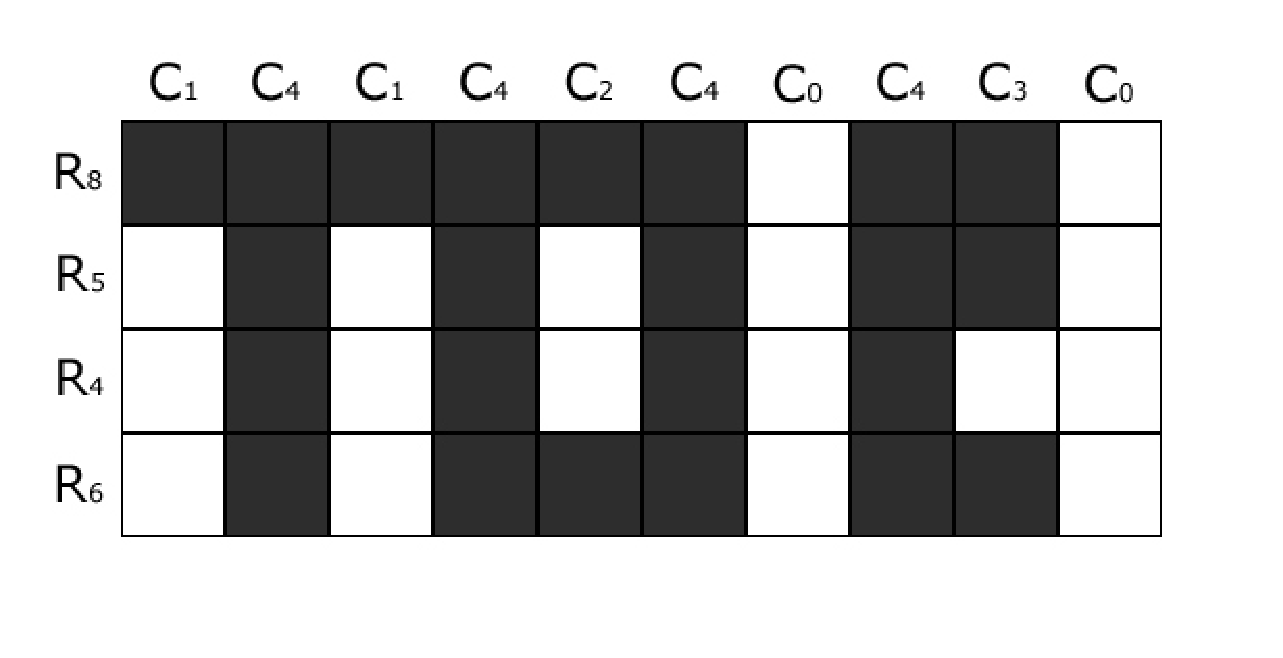
\includegraphics[height=5cm]{equiv_classes_example}
\caption{Equivalence classes of a black and white pattern P.}
\label{fig:equiv_classes_example}
\end{figure}

Note that every row and column belongs to exactly one equivalence class. Also, if two columns belong to a equivalence class in the beginning of the MPUS algorithm, they will remain of the same class until one of them is picked up
by the algorithm. This is since picking up other columns does not
change these two columns at all, while picking up rows modify these
two columns in exactly the same way. The same property holds for two
rows that belong to a equivalence class.

 %the very end of its execution. This will be proven later,
 %but the idea is that if any cell of row or column is removed,
 % the same cell will be removed for every member of its equivalence class.

We also define an equivalence class as being {\em active} during the execution of the MPUS algorithm if some member of that class is pseudo-monochromatic
but not all gray.

\subsubsection{Active Classes Properties.}
"Applegate et al."'s paper shows that during the execution of the MPUS algorithm on a black and white strip-rule pattern, there are always exactly two active classes at any given time.
The intuition on why this happens is that in order for a new class to become active, all the members of an old active class need to be picked up.
A formal proof of this property appears later in
Proposition \ref{t_active_classes} in the Appendix
(Subsection \ref{ss_classes});
this fact is also used in \cite{ACJKLW07}.
Also, the same proposition shows that
the two active classes are either a row and a column
class of the same color or both classes of the same kind (rows or columns),
 being one of each color.

\subsubsection{Embedded Rows and Columns.}
We can start improving the MPUS algorithm by introducing the concept described by "Applegate et al."'s paper as embedded rows and columns. This will allow us to pick up more rows and columns using the same number of rectangles.

First, we will define the concept of a embedded column or row at a given stage of the MPUS algorithm.
Given a point during the execution of the MPUS algorithm,
let $b$ be a column of an active equivalence class $B$.
Let $a_{1}$ be the first column to the left of $b$ that does not belong to $B$ and has not yet been picked up.
Similarly, let $a_{2}$ be the first column to the right of $b$ that does not belong to $B$ and has not yet been picked up.
We say that $b$ is {\em embedded}
 in equivalence class $A$ if both $a_{1}$ and $a_{2}$ belong to that class $A$. The definition is analogous for rows. Note that columns can be embedded only in column classes and rows only in row classes. See the three leftmost columns of Fig.~\ref{fig:embedment_example} for a simple example of a white column embedded in two black columns.

\begin{figure}[h]
\centering
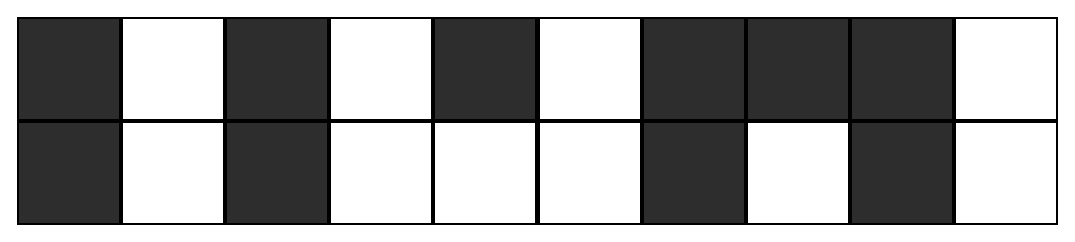
\includegraphics[width=10cm]{embedment_example}
\caption{Example of a pattern $P$ where some members of $C_{0}$ are embedded in some members of $C_{2}$.}
\label{fig:embedment_example}
\end{figure}

If during the execution of the MPUS algorithm we have the option to pick up two
column-blocks that embeds a set of columns of another class,
 we could pick up the two column-blocks that embeds the third one with
 two rectangles and then the embedded one, totaling three rectangles.
 However, it is better to pick the embedded block first with one rectangle,
and then pick the two blocks that were previously embedding with only one
rectangle, thus using a total of two rectangles for the same set of columns.
As an example, in Fig.~\ref{fig:embedment_example}, one cannot benefit
by picking up the first and the third column, when one can pick up
first the second column, followed by picking up the block of the first three
columns.

\subsubsection{Equivalence Classes Ordering.}
\label{ss_ordering}
As we pick up all the members of a column class, we change the rows of the pattern. Since the other columns remain intact, the new class to become active must be a row class. By using the same argument for row classes, we see that whenever we pick up all the members of a class, the next class to become active is of the opposite type.  This is formally proven in Proposition
\ref{theorem_pick_up_altertation} in the Appendix.
Also (same proposition), if we pick up all the members of an active class that was pseudo-monochromatic on a given color (for instance, black), the next class to become active needs to be of the opposite color (for instance, white). This happens because if it was of the same color, the other class would already have been active.

We can order the equivalence classes of both rows and columns in a given
 pattern $P$ by the number of black cells on it. In that ordering,
we can see (Proposition \ref{theorem_difference_is_class} in the Appendix)
that the all the rows that two consecutive column classes differ
 form exactly an equivalence class. This holds analogously for columns.
This implies (Proposition \ref{lemma_num_rows_col_differ_one} in the Appendix)
that the numbers of columns and rows classes differ
by at most one.  Using that information,
 we can set up the following ordering for the equivalence classes
(see also Proposition \ref{corollary_hierarchical_sequence} in the Appendix):

\begin{enumerate}

\item Start with the column class with only white cells. If such class does not exist, start with the row class with only black cells  (the existence of
this row class follows immediately from the monotonicity property -
Theorem \ref{theorem_strip_rule_patterns} in the Appendix).

\item Alternate columns and rows, putting the columns in ascending order of black cells and the rows in descending order of black cells.

\end{enumerate}

Let $C_{x_{0}}, C_{x_{1}}, \cdots, C_{x_{(N_{C}-1)}}, C_{x_{N_{C}}}$ be the ascending ordering of column classes by the number of black cells. Let $R_{y_{0}}, R_{y_{1}}, \cdots, R_{y_{(N_{R}-1)}}, R_{y_{N_{R}}}$ be the ascending ordering of row classes by the number of black cells. Using the rules above, we should get an ordering similar to $C_{x_{0}}, R_{y_{N_{R}}}, C_{x_{1}}, R_{y_{(N_{R}-1)}}, \cdots, R_{y_{1}}, C_{x_{(N_{C}-1)}}, R_{y_{0}}, C_{x_{N_{C}}}$. We will call this ordering the {\em hierarchical array} of the pattern $P$. We will also refer to this ordering of equivalence classes as $E_{1}, E_{2}, \cdots, E_{N}$.
Note that $N_C$, the number of column classes, is at most $n_C$,
the number of columns, and the same property holds for rows.

One important property of the hierarchical array of a pattern is that if $E_{x}$ and $E_{y}$, $x < y$, are the active classes during the MPUS execution, all classes that come before $E_{x}$ in the sequence or after $E_{y}$ must have already been picked up (otherwise, $E_{x}$ and $E_{y}$ would not be active).
This is proven in Proposition \ref{corollary_hierarchical_sequence}
in the Appendix.
Also from \ref{corollary_hierarchical_sequence}, if a class is between those two classes, none of the rows/columns of the in-between class
are pseudo-monochromatic.
The hierarchical array is a useful extension of Observation 5 on page
1070 of \cite{ACJKLW07}.


\subsection{Segments}

During MPUS, there are always two active classes. A ``segment"
succinctly represents the blocks that are available for pick up
while a certain pair of classes are active.
These segments can be translated into nodes of a graph, that can be used for finding the optimal solution, as described below. Note that our representation of segments is a slightly condensed version of the one described in the original
"Applegate et al."'s paper \cite{ACJKLW07}. The difference is that
the original definition is a five tuple with two redundant fields.
See Subsection \ref{ss_seg} of the appendix for a proof that these fields are
redundant. It is not here where the running time is improved.

\subsubsection{Definition and Properties.}

Whenever a new class becomes active during the execution of the MPUS algorithm
 on a pattern $P$, we will define a {\em segment} $S$ as being a tuple of
three elements $(E_{x},E_{y},U)$ where $E_{x}$ and $E_{y}$ are the active
equivalence classes and $U$ is the subset of members (rows or columns)
 left unpicked of $E_{y}$ ($U \subset E_{y}$).

We can represent the sequence of actions of the MPUS execution as
a sequence of segments, as described in this paragraph.
 Given the pick-up order obtained through the execution of the MPUS,
let's create a segment $(E_{0}, E_{N}, E_{N})$ for the starting state of pattern $P$ and a segment $(E_{x}, E_{y}, U)$, $U \subset E_{y}$, for every time a new class $E_{x}$ becomes active; we say that the SRRL {\em includes} the
segment whenever such a segment becomes active during the MPUS execution
corresponding to the SRRL.

Since $E_{x}$ is the new class, all of the members of $E_{x}$ are still in the pattern. $E_{y}$, in the other hand, is a class that was already active. It may have some of its members already picked-up. We store that information in $U$ by maintaining the members that have not been picked up yet. Note also that any classes that are between $E_{x}$ and $E_{y}$ in the hierarchical array of $P$ have not become active yet, resulting in the fact that all of
their members are still there. At the same time, members that come before and after the interval delimited by $E_{x}$ and $E_{y}$ have all been picked up. Hence, for each one of those segments that are created whenever a class becomes active it is possible to reconstruct the pattern at that moment of the execution of the MPUS algorithm.

\subsubsection{Segment Branching.}

"Applegate et al."'s paper \cite{ACJKLW07}
shows that if we are looking for an optimal solution we can narrow down the number of segments significantly by reducing the number of options a segment can branch to two.

Suppose a minimum-length SRRL for a strip-rule pattern $P$ includes the segment $S = (E_{x}, E_{y}, U)$ and that to get to the next segment, if it exists, we pick up all members of $E_{x}$
(possibly picking up some members of $U \subset E_{y}$)
while at least one member of $U$ remains active.

\begin{itemize}

\item If $U \subset E_{y}$ has a member that is not embedded in $E_{x}$,
 there exists a minimum-length SRRL that includes the segment
$S = (E_{x}, E_{y}, U)$ and that to get to the next segment you pick up
 all the members of $U \subset E_{y}$ that are embedded in $E_{x}$,
 followed by picking all members of $E_{x}$.

\item If all members of $U \subset E_{y}$ are embedded in $E_{x}$,
 there exists another minimum-length SRRL that includes the segment
$S = (E_{x}, E_{y}, U)$ and that to get to the next segment you
 pick up all the members of $U \subset E_{y}$
(thus, finishing picking up every member of $E_{y}$ in the pattern).
Note that in this case, one can get to the next segment by picking up all
the members of $U \subseteq E_y$ first.

\end{itemize}

The same property holds with the roles of $E_{x}$ and $U$ switched. In this case, we assume the next segment from $S$, if it exists is originally reached by picking up all members of $U \subset E_{y}$.

This happens because we can always pick embedded members at no extra cost,
if one is to pick all the blocks of the embedding class, as shown in
Proposition \ref{p_embed} of the Appendix.
Moreover, suppose we have two sets $U_x$ and $U_y$
of active blocks of the two active classes $E_x$ and $E_y$.
To finish picking up blocks (except at the very end), we must
reach the situation that either $E_x$ or $E_y$ are not active anymore;
say $E_x$ becomes not active, while $E_y$ is still active.
%together with a new active class $E_z$.
Picking up any block from the class $E_y$ that is not embedded in $E_x$
can be done, without loss of optimality, later.
So we can assume that
 only the members of $U_y$ that are embedded in $E_x$ are picked up
while $E_x$ is active.

 Note also that for every segment we could pick the latest class that became active or the oldest, a total of two options. We can then say that every segment will branch into two other segments. On both cases, we can determine the next segment reached by eliminating every embedded member of the class not being picked-up, followed by eliminating every member of the class being picked-up. The only exception to this, is if when we pick every embedded member of the class not being picked-up we end up picking all of its members, thus already reaching a new segment. In that case, the original segment branches into only one segment, instead of two.

Note that there could be a segment that does not have any next segment. In this case, the segment is a segment at the very end of minimum-length SRRL. If we pick up any of either class, we will obtain an all-gray grid and the algorithm will be over. Also, note that for this to happen we must have that $E_{x}$ and $E_{y}$ are next to each other in the hierarchy array, and picking-up one of them will also result in picking-up the other one.

\subsubsection{Segment Graph.}

We build a graph using the segments as nodes, as described by the following structure proposed by \cite{ACJKLW07}:

\begin{itemize}

\item Start with the segment $(E_{0}, E_{N}, E_{N})$, that represents the grid as it is in very beginning of the MPUS algorithm. This will be the starting node.

\item For every node (segment) in the graph, generate the two segments (possibly one, as described in the previous subsection) that it branches into and add a directed edge from it to the new generated nodes.
 There will be one segment for each of the two options of picking up the newest or the oldest of the two classes in the segment. On both cases, we can determine the next segment reached by eliminating every embedded member of the class not being picked-up, followed by eliminating every member of the class being picked-up.

\item Define the cost for each edge as the number of rules in the MPUS algorithm used to go from one segment to another.

\item Create an artificial node corresponds to an all-gray grid. This will be the end node of the graph. Every time a segment has its two classes adjacent to each other in the hierarchy array, create an edge from it to this all-gray grid node.
 This edge should have cost one (since we solve the modified version);
if we were to solve the original version, this edge should have cost zero
if the members of the classes of the segment were white and one otherwise.

\end{itemize}

Because of what was discussed in the Segments Branching section, at least one of the paths from the starting node to the end node of the graph will be a minimum-length SRRL.
 Note that having $(E_{N}, E_{0}, E_{0})$ as the starting node will lead to a graph that represents the same possible steps for the MPUS because it also represents the same starting pattern. Note also that some nodes may be reached by more than one node. Every node will only branch into nodes that correspond to patterns with fewer total of columns and rows. This implies that there are no cycles in this graph.

We say that one segment reaches another if there is a path in this graph from that segment to the other one. The distance from one segment to another is the sum of the costs of the edges that compose the path between them, if such exists.

One very important property of this graph that will be proven later is that if two segments $(E_{x}, E_{y}, U)$ and $(E_{x}, E_{y}, U')$ are reachable from the the starting node of the graph, then either $U \subset U'$ or $U' \subset U$. This property will be referred as the Containment Lemma and appears
in Subsection \ref{ss_cont} in the Appendix. We will see that this implies that the number of nodes in this graph is $O(n^{2})$ where $n$ is the number of rows and columns in the original pattern.




